% Venn options: 2x2 panels, U boxes, M/N relations preserved.
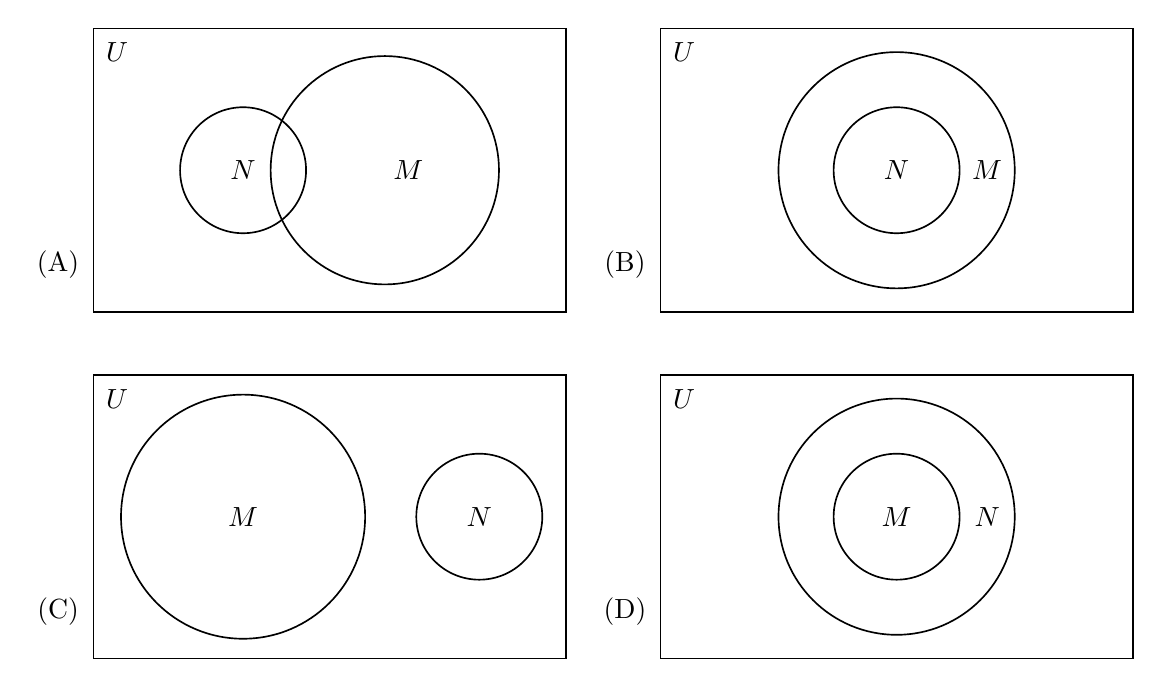
\begin{tikzpicture}[line width=.6pt,font=\normalsize]
% Panel A: N small intersects M large
\begin{scope}[shift={(-3.6,2.2)}]
\draw (-3,-1.8) rectangle (3,1.8);
\draw (-1.1,0) circle (0.8);
\draw (0.7,0) circle (1.45);
\node at (-1.1,0) {$N$};
\node at (1.0,0) {$M$};
\node at (-2.7,1.5) {$U$};
\node at (-3.45,-1.2) {(A)};
\end{scope}
% Panel B: N inside M
\begin{scope}[shift={(3.6,2.2)}]
\draw (-3,-1.8) rectangle (3,1.8);
\draw (0,0) circle (1.5);
\draw (0,0) circle (0.8);
\node at (0,0) {$N$};
\node at (1.15,0) {$M$};
\node at (-2.7,1.5) {$U$};
\node at (-3.45,-1.2) {(B)};
\end{scope}
% Panel C: M and N disjoint
\begin{scope}[shift={(-3.6,-2.2)}]
\draw (-3,-1.8) rectangle (3,1.8);
\draw (-1.1,0) circle (1.55);
\draw (1.9,0) circle (0.8);
\node at (-1.1,0) {$M$};
\node at (1.9,0) {$N$};
\node at (-2.7,1.5) {$U$};
\node at (-3.45,-1.2) {(C)};
\end{scope}
% Panel D: M inside N
\begin{scope}[shift={(3.6,-2.2)}]
\draw (-3,-1.8) rectangle (3,1.8);
\draw (0,0) circle (1.5);
\draw (0,0) circle (0.8);
\node at (0,0) {$M$};
\node at (1.15,0) {$N$};
\node at (-2.7,1.5) {$U$};
\node at (-3.45,-1.2) {(D)};
\end{scope}
\end{tikzpicture}
